\documentclass{article}

% Language setting
% Replace `english' with e.g. `spanish' to change the document language
\usepackage[english]{babel}

% Set page size and margins
% Replace `letterpaper' with `a4paper' for UK/EU standard size
\usepackage[a4paper,top=2cm,bottom=2cm,left=3cm,right=3cm,marginparwidth=1.75cm]{geometry}

% Useful packages
\usepackage{amsmath}
\usepackage{graphicx}
\usepackage[colorlinks=true, allcolors=blue]{hyperref}
\usepackage{float}
\usepackage{wrapfig}
\title{MF6RTM: Reactive Transport Model via the MODFLOW 6 and PHREEQCRM APIs}
\author{Pablo Ortega, Ed de Sousa and Jeremy White}

\begin{document}
\maketitle


\section{Integration Overview}
This integration leverages the modular capabilities of MF6 with the geochemical reaction capabilities of PHREEQC. Here’s a brief description of how the coupling is currently working:

\begin{itemize}

    \item \textbf{Initialization}: The function begins by initializing the PHREEQCRM and corresponding arrays from a phinp.dat file (PHREEQC file generated from dictionaries).

    \item \textbf{MF6 Model Setup}: Retrieves the grid dimensions from the MF6 dis object. It identifies and lists the components being transported, which are derived from the PHREEQCRM components. It then writes the MF6 model files for each component.
    
    \item \textbf{Transport Solution Loop}: For each time step, the function prepares MF6 for solving and runs the transport model. The function handles potential convergence issues by tracking and reporting iterations and failures.
    
    \item \textbf{Reaction Calculations}: If reactions are enabled, arrays are sent to PHREEQCRM which runs the cell reactions and retrieves the resulting concentrations. These concentrations are then converted and set back into MF6.
    
    \item \textbf{Output}: Outputs as UCN are being handled by MF6 but user-defined selected outputs can also be included and saved as csv.

\end{itemize}

The current version is intended to work with structured grids (dis object in MF6) and one MF6 simulation that includes the flow and transport solutions. No support is currently provided for a 'flow then transport scheme,' meaning that advanced packages cannot be incorporated yet. On the PHREEQC side, the following have been included:

\begin{itemize}
    \item  Solution
 \item Equilibrium phases
 \item Cation Exchange
 \item Surface Complexation
 \item Kinetics
\end{itemize}

\section{Benchmarks}

\subsection{Example 1 - Engesgaard and Kipp 1992}

The case described in Example 1 was originally presented by Engesgaard and Kipp (1992) for a model verification of their MST1D code against the CHEMTRNS model by Noorishad et al. (1987). It involves a one-dimensional model domain in which an aqueous water composition that is in equilibrium with two minerals, calcite and dolomite, is successively replaced, i.e., flushed by water of a different chemical composition, leading to multiple precipitation-dissolution fronts. Dolomite is not present initially but is formed temporally. Transport in MF6 was simulated using the WEL package with auxiliary variables and the SSM package. Benchmarks against PHT3D are presented in Figure \ref{fig:ex1}.




\begin{figure}[H]
\centering

    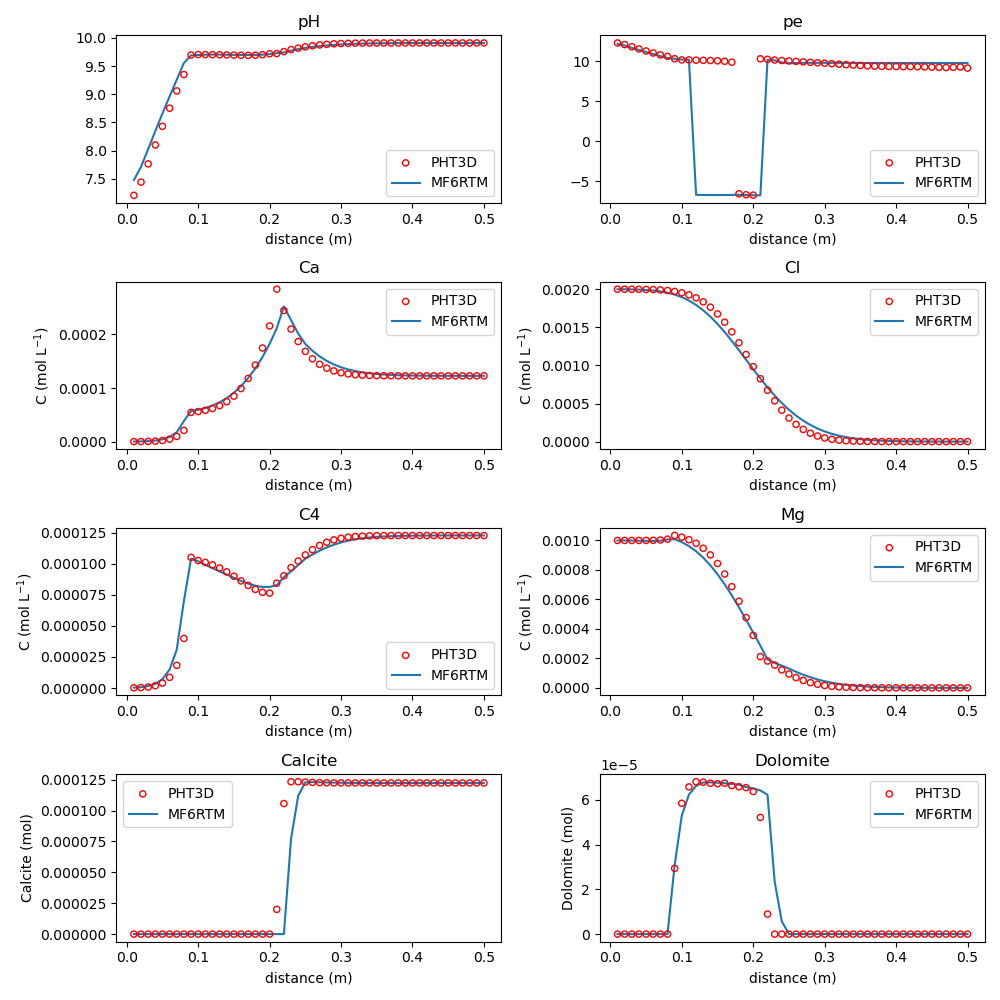
\includegraphics[width=\linewidth]{figures/ex1.png}
\caption{ Engesgaard 1992. MF6RTM vs PHT3D.}
\label{fig:ex1}
\end{figure}

\subsection{Example 2 - Walter 1994 in 1D. Migration of precipitation/dissolution fronts}

This test problem is a one-dimensional, purely inorganic redox problem that was first presented by Walter et al. (1994). It was subsequently used as a benchmark problem by Guerin and Zheng (1998). It demonstrates the evolution of some important geochemical processes that occur when acidic mine tailings leach into an anaerobic carbonate aquifer. Aqueous complexation and dissolution/precipitation are all considered equilibrium reactions. If the reaction network defined by Walter et al. (1994) is used, the simulation includes 17 aqueous components, 15 of which are transported, 54 aqueous species, and six minerals. Transport in MF6 was simulated using the WEL package with auxiliary variables and the SSM package. Benchmarks against PHT3D are presented in Figure \ref{fig:ex2}. Time stepping for MF6RTM is ten times that of PHT3D to achieve similar results due to numerical dispersion.

\begin{figure}[H]
\centering

    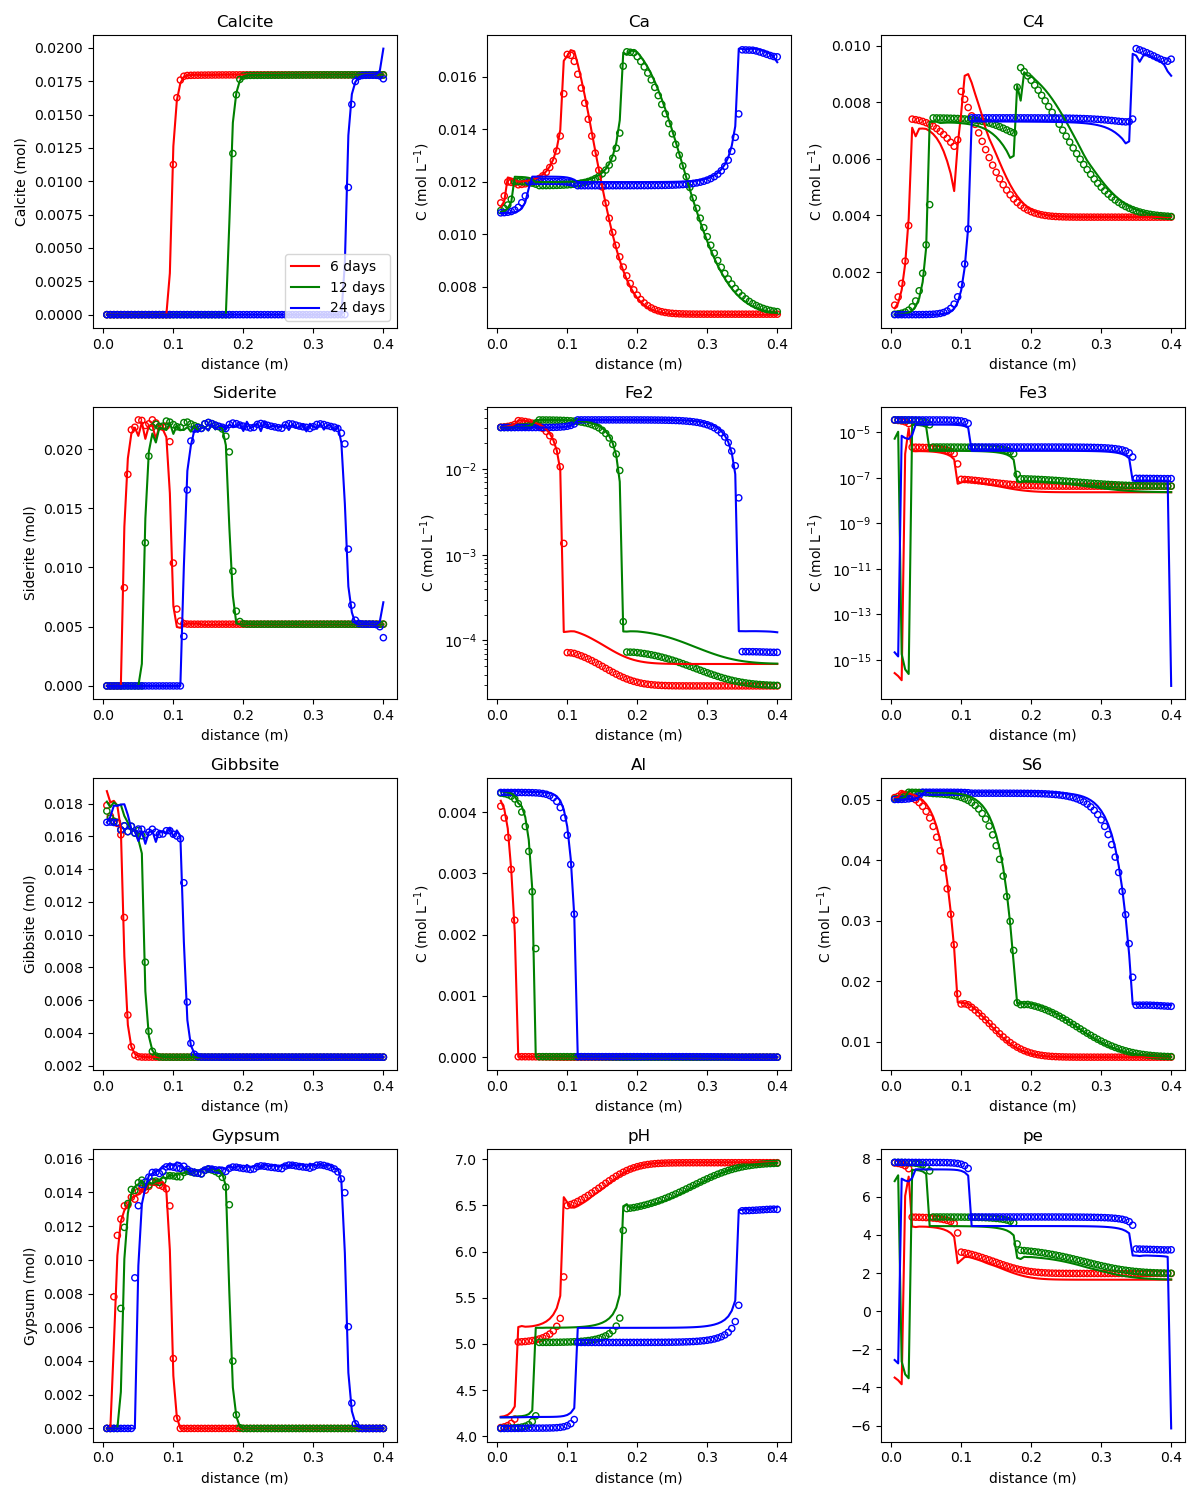
\includegraphics[width=\linewidth]{figures/ex2_10xtsteps.png}
\caption{Walter 1992. Precipitation/dissolution 1D front. MF6RTM (lines) vs PHT3D (circles).}
\label{fig:ex2}
\end{figure}


\subsection{Example 3 - Walter 1994 in 2D. Migration of precipitation/dissolution fronts}
This problem is the same as in Example 2 but in two dimensions. The original PHT3D version of this model employs the SSMS package linked to the WEL package, in addition to CNC to represent the aquifer. A similar setup was built for MF6 using CHD with auxiliary variables and CNC.
\begin{figure}[H]
\centering

    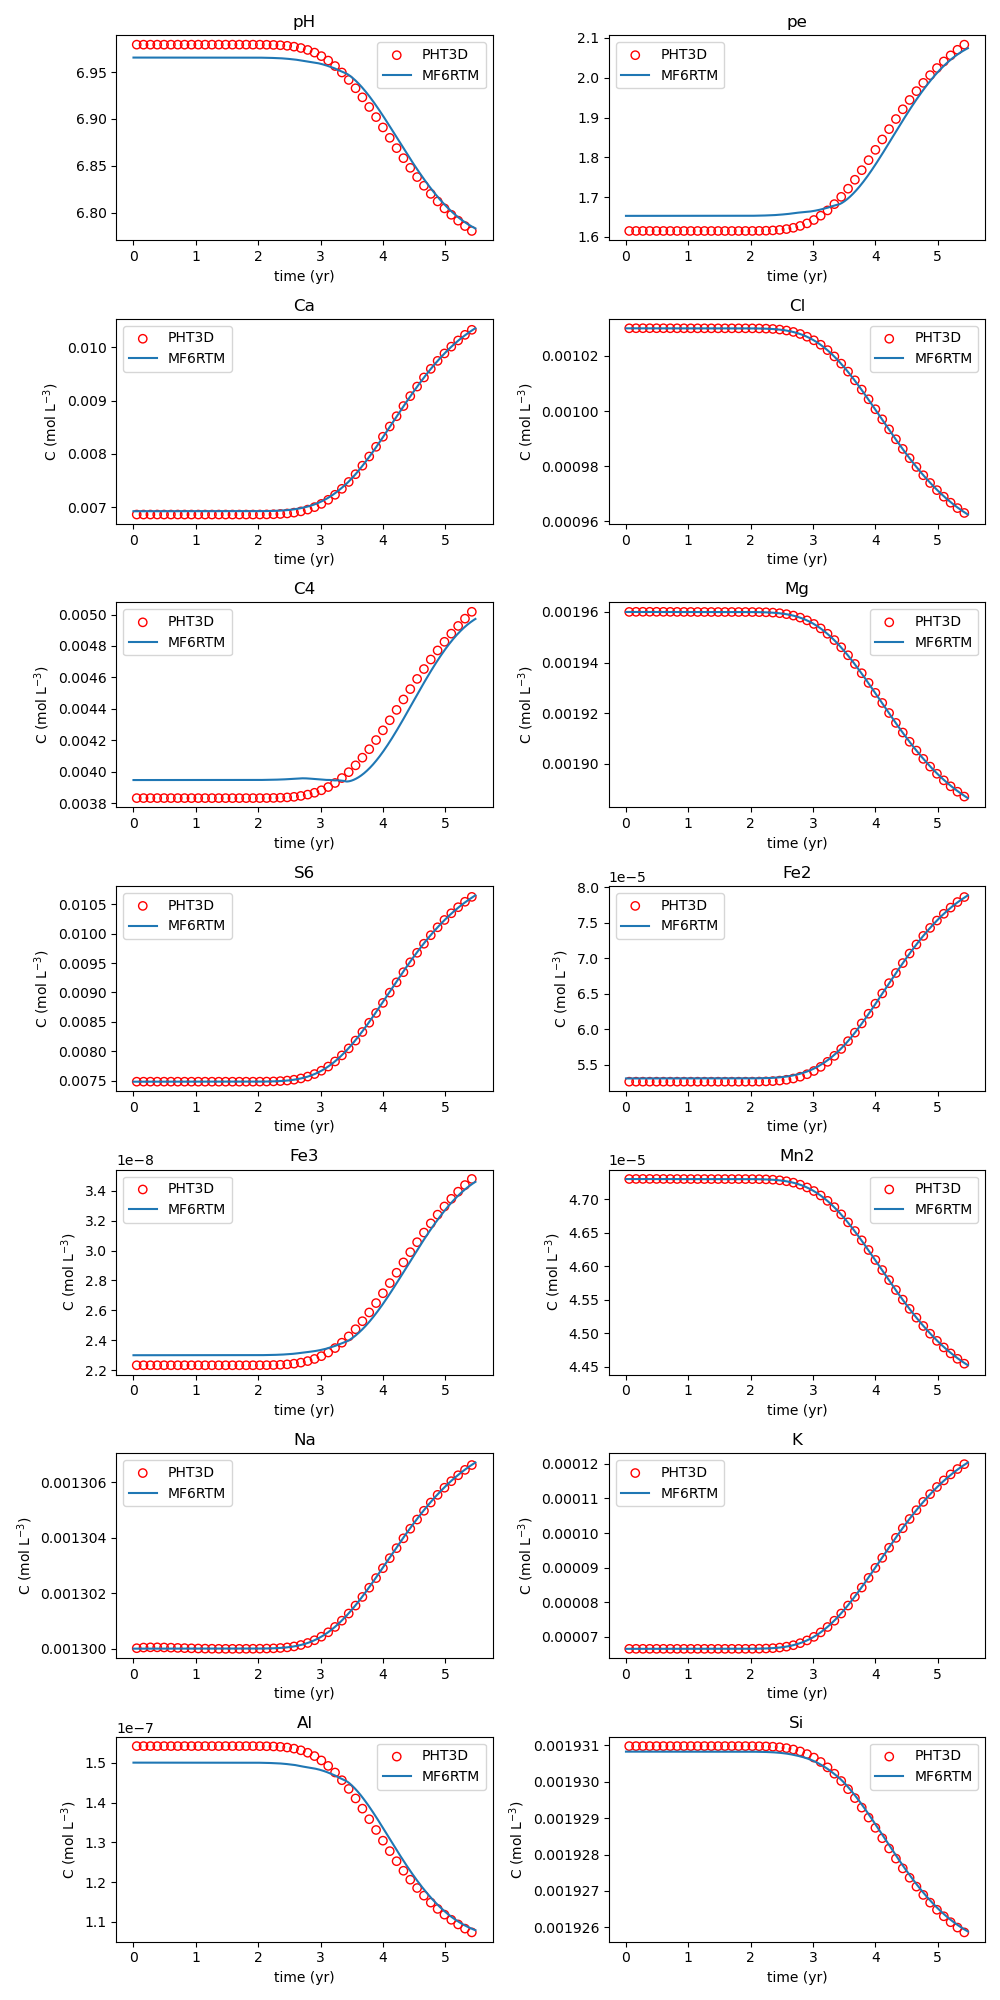
\includegraphics[width=0.8\linewidth]{figures/ex3.png}
\caption{Walter 1992 2D benchmark. Precipitation/dissolution 2D front. MF6RTM (lines) vs PHT3D (circles).}
\label{fig:ex3_1}
\end{figure}

\begin{figure}[H]
\centering

    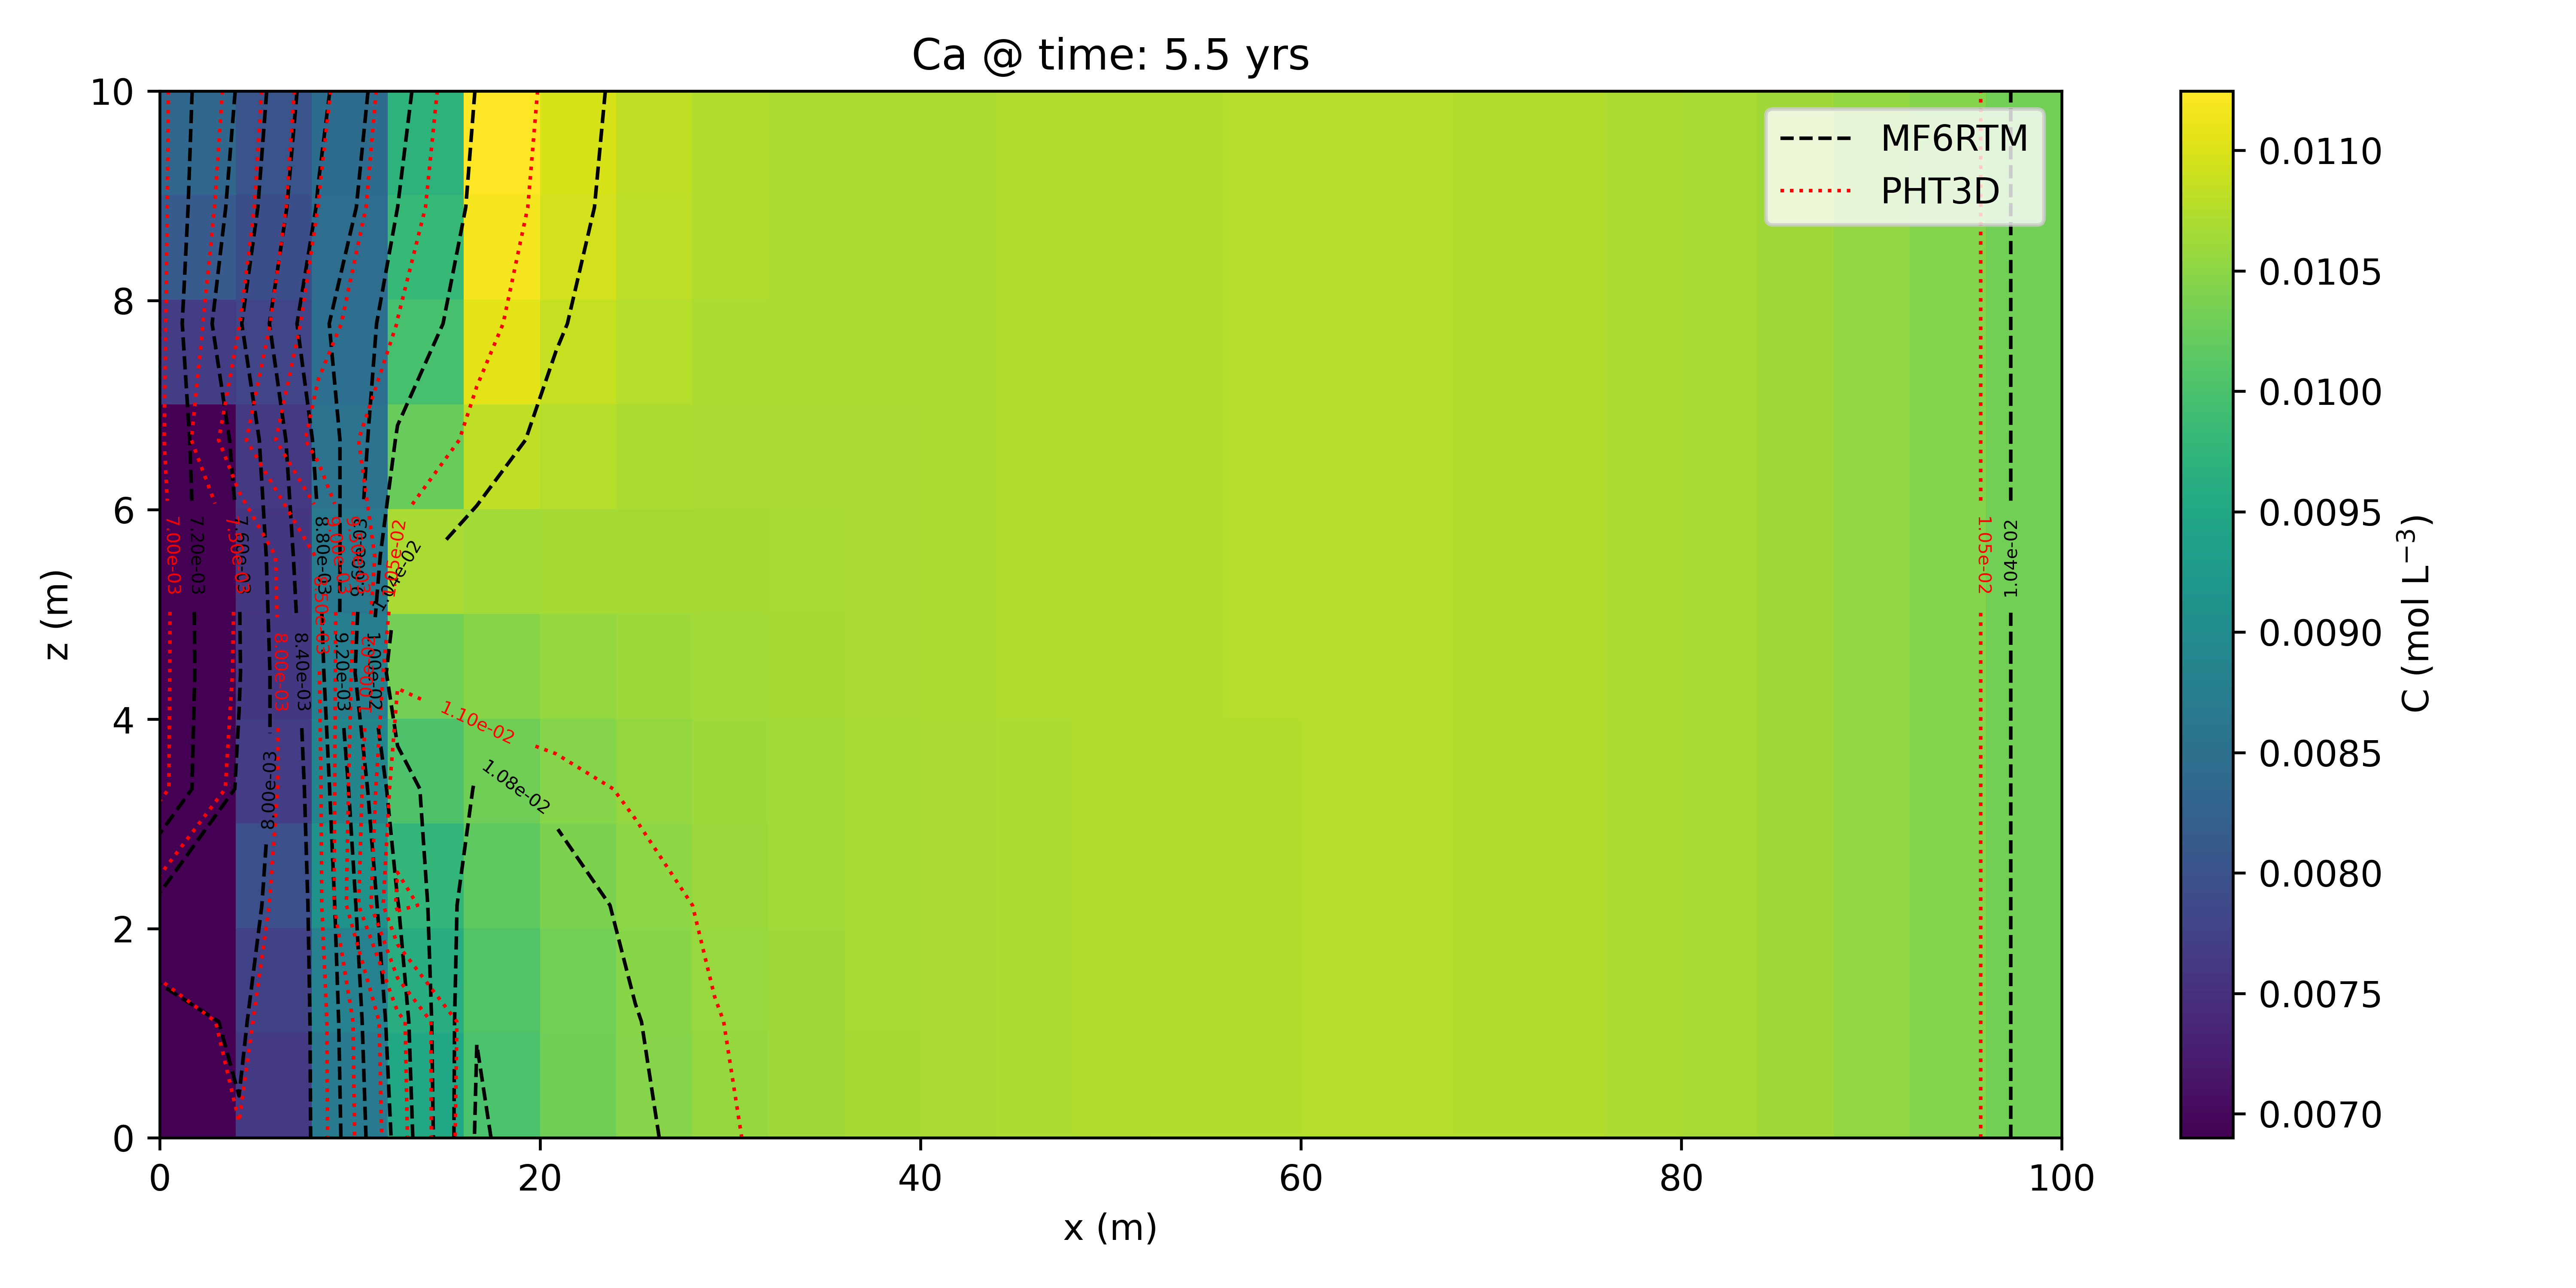
\includegraphics[width=\linewidth]{figures/ex3_Ca_2000.png}
\caption{Walter 1992 2D benchmark. Cross-section map. Precipitation/dissolution 2D front.}
\label{fig:ex3_2}
\end{figure}

\subsection{Example 4 - Cation exchange- flushing of a sodium-potassium nitrate solution with calcium chloride}
This benchmark demonstrates ion-exchanging reactions in flow-through systems. The example was originally used as a PHREEQM (Nienhuis et al., 1994) test case and is also included in the PHREEQC-3 documentation (Parkhurst and Appelo, 2013) as Example 11. Further discussion can be found in Appelo and Postma (1993), where it forms Example 10.13, and in Appelo (1994). The one-dimensional simulation problem describes a hypothetical column experiment where porewater containing sodium (\(\text{Na}^+\)), potassium (\(\text{K}^+\)), and nitrate (\(\text{NO}_3^-\)) in equilibrium with exchangeable cations was flushed by a calcium chloride (\(\text{CaCl}_2\)) solution. This example is benchmarked against PHT3D and PHREEQC-3. The time-stepping scheme for MF6RTM is twice that used by PHT3D and PHREEQC to achieve similar results due to numerical dispersion.



\begin{figure}[H]
\centering

    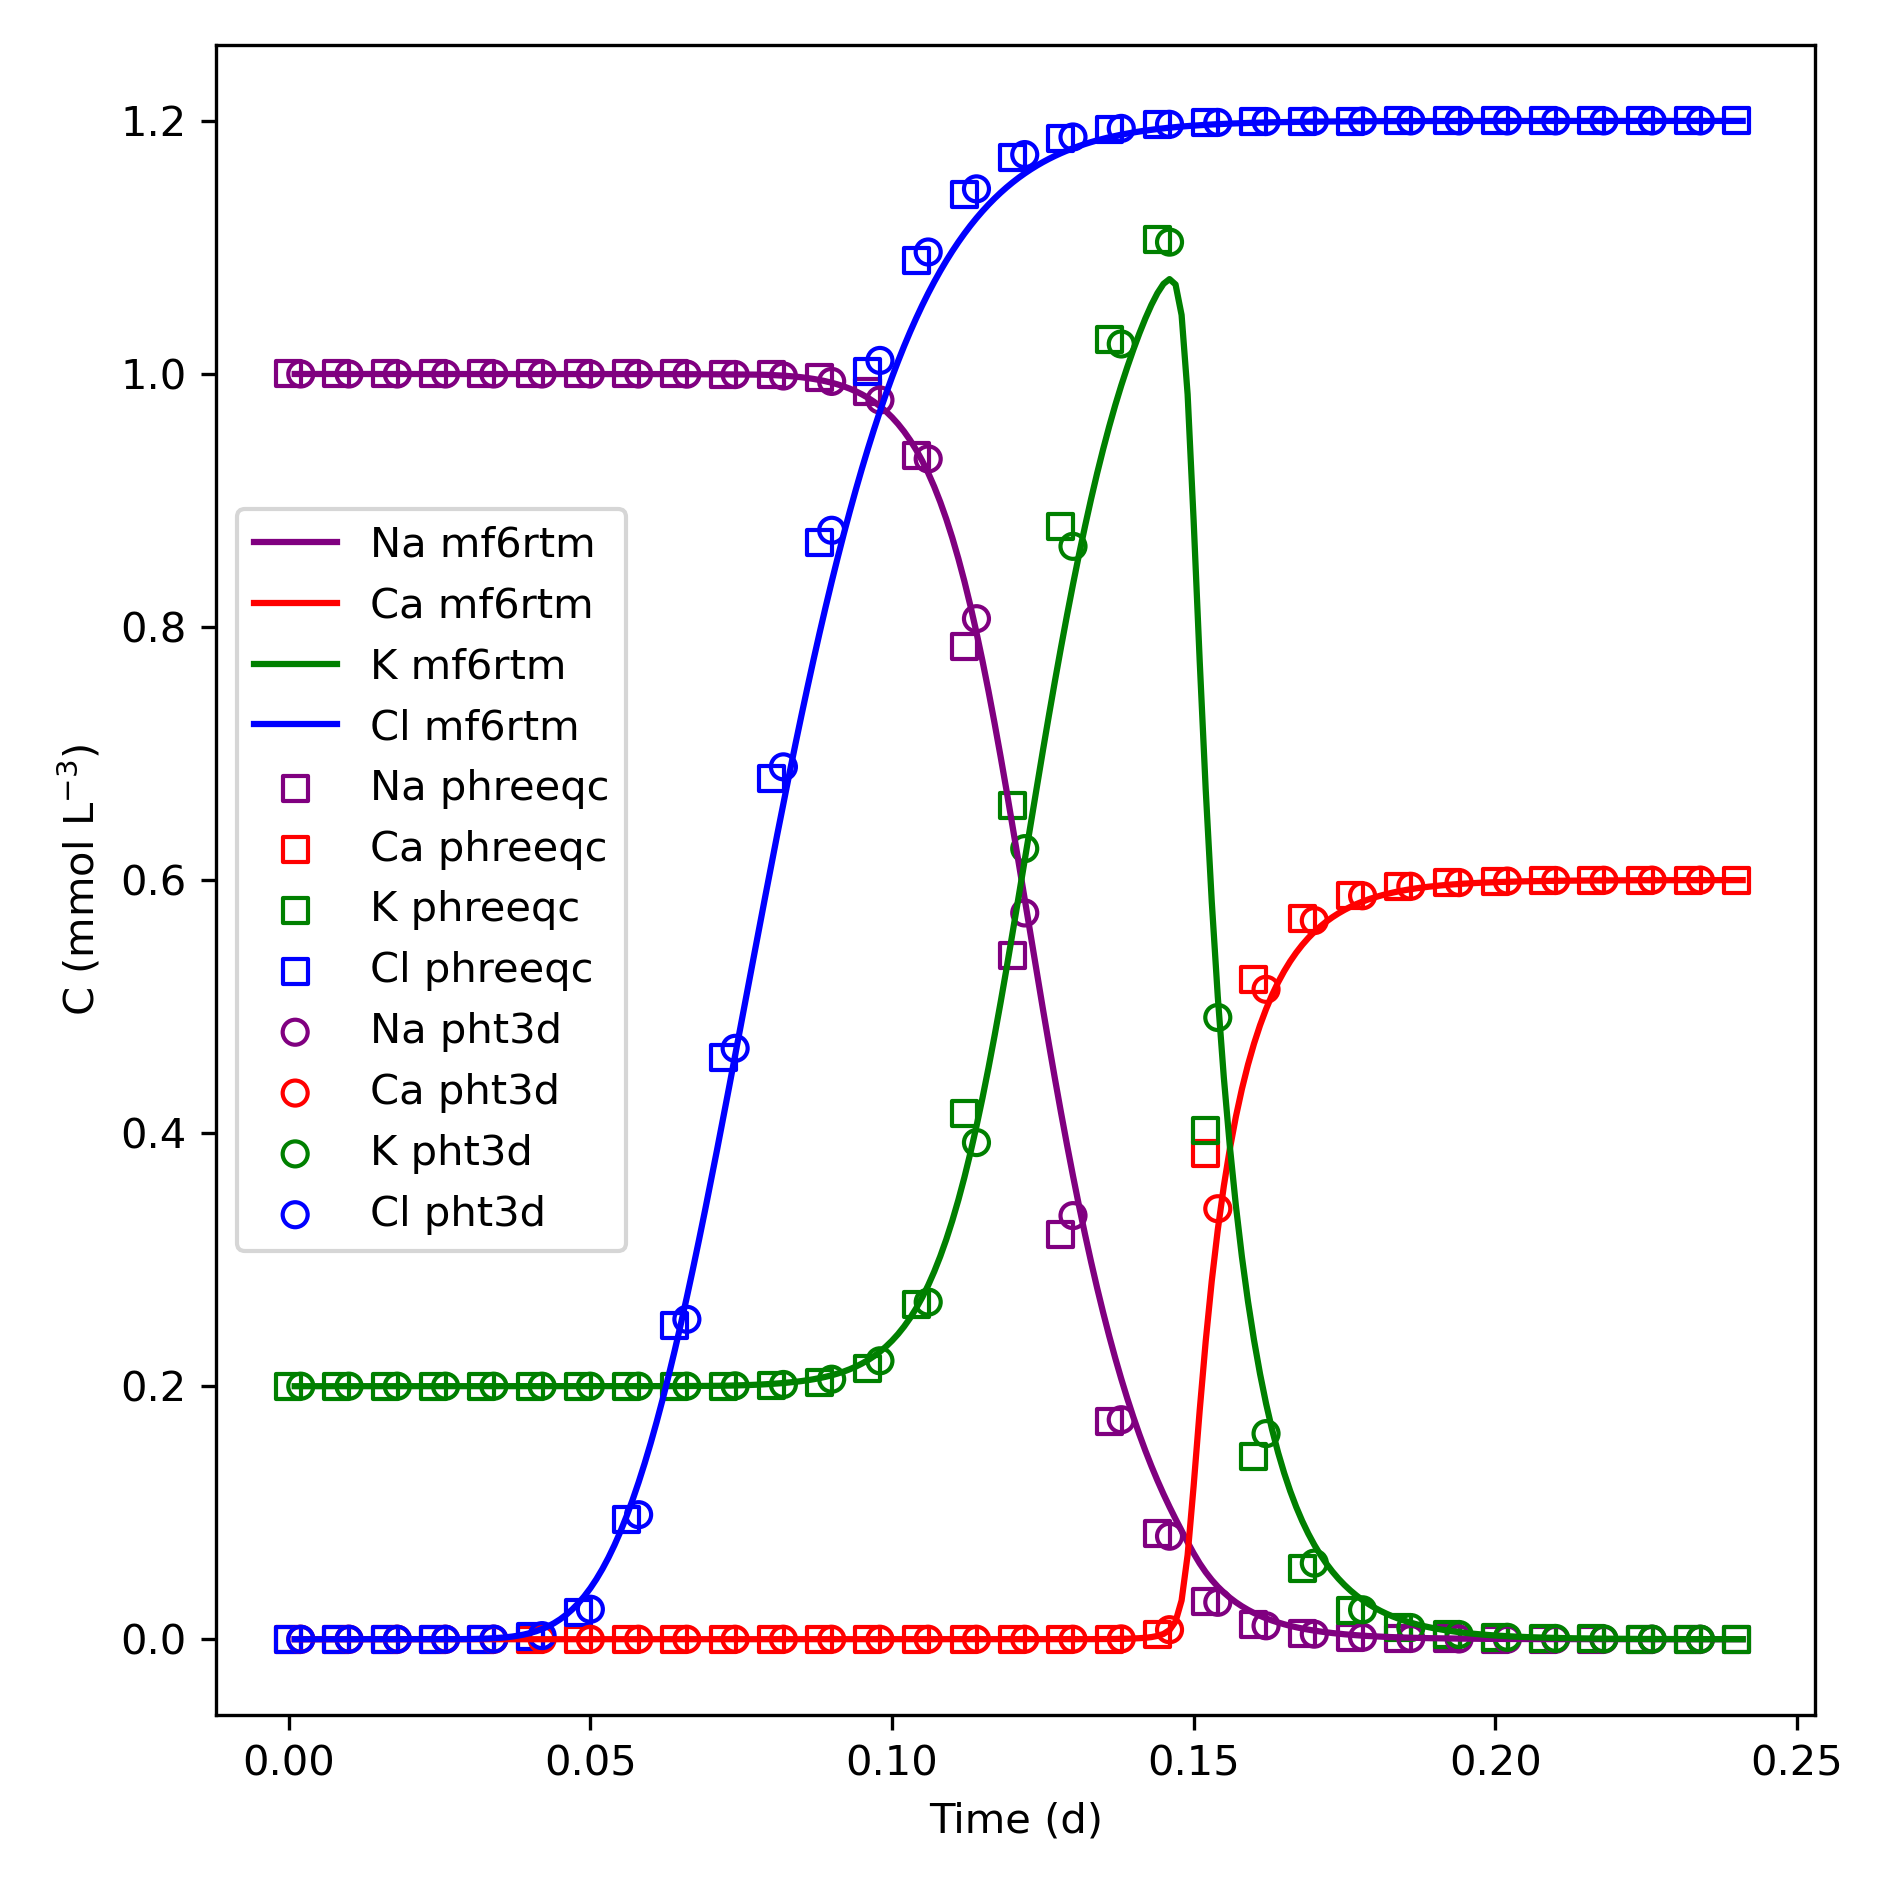
\includegraphics[width=0.8\linewidth]{figures/ex4.png}
\caption{Cation Exchange 1D. MF6RTM vs PHT3D and PHREEQC.}
\label{fig:ex4}
\end{figure}


\subsection{Example 5 - Oxidation Experiment using using a combination of equilibrium phases, kinetic and rates, cation exchange, and surface complexation}
This benchmark describes the simulation of an oxidation experiment with marine pyrite-containing sediments. This model and the experimental work were originally reported by Appelo et al. (1998). The conceptual hydrochemical model and the implemented reaction network proposed for this experiment comprise a complex set of reactive processes. This includes:

\begin{itemize}
    \item the oxidation of pyrite, which is the primary driver of hydrochemical changes,
    \item secondary reactions, such as dissolution of calcite, CO$_2$ sorption, cation and proton exchange, and
    \item oxidation of organic matter, a reaction that competes for the oxidation capacity supplied by the inflow solution.
\end{itemize}

The model considers three distinct phases of the experiment. In the first part, the sediment material collected in the field was equilibrated with a 280 mmol MgCl$_2$ solution. In this phase, the pore space becomes filled with the MgCl$_2$ solution and the exchanger sites are filled with Mg. In the second phase, the column was fed with a more dilute MgCl$_2$ solution, while in the third phase, the column was flushed for 4 pore volumes (at the same flow rate) with a hydrogen peroxide (H$_2$O$_2$) containing oxidizing solution. This benchmark illustrates the behavior of MF6RTM using a combination of equilibrium phases, kinetic and rates, cation exchange, and surface complexation without EDL.
\begin{figure}[H]
\centering

    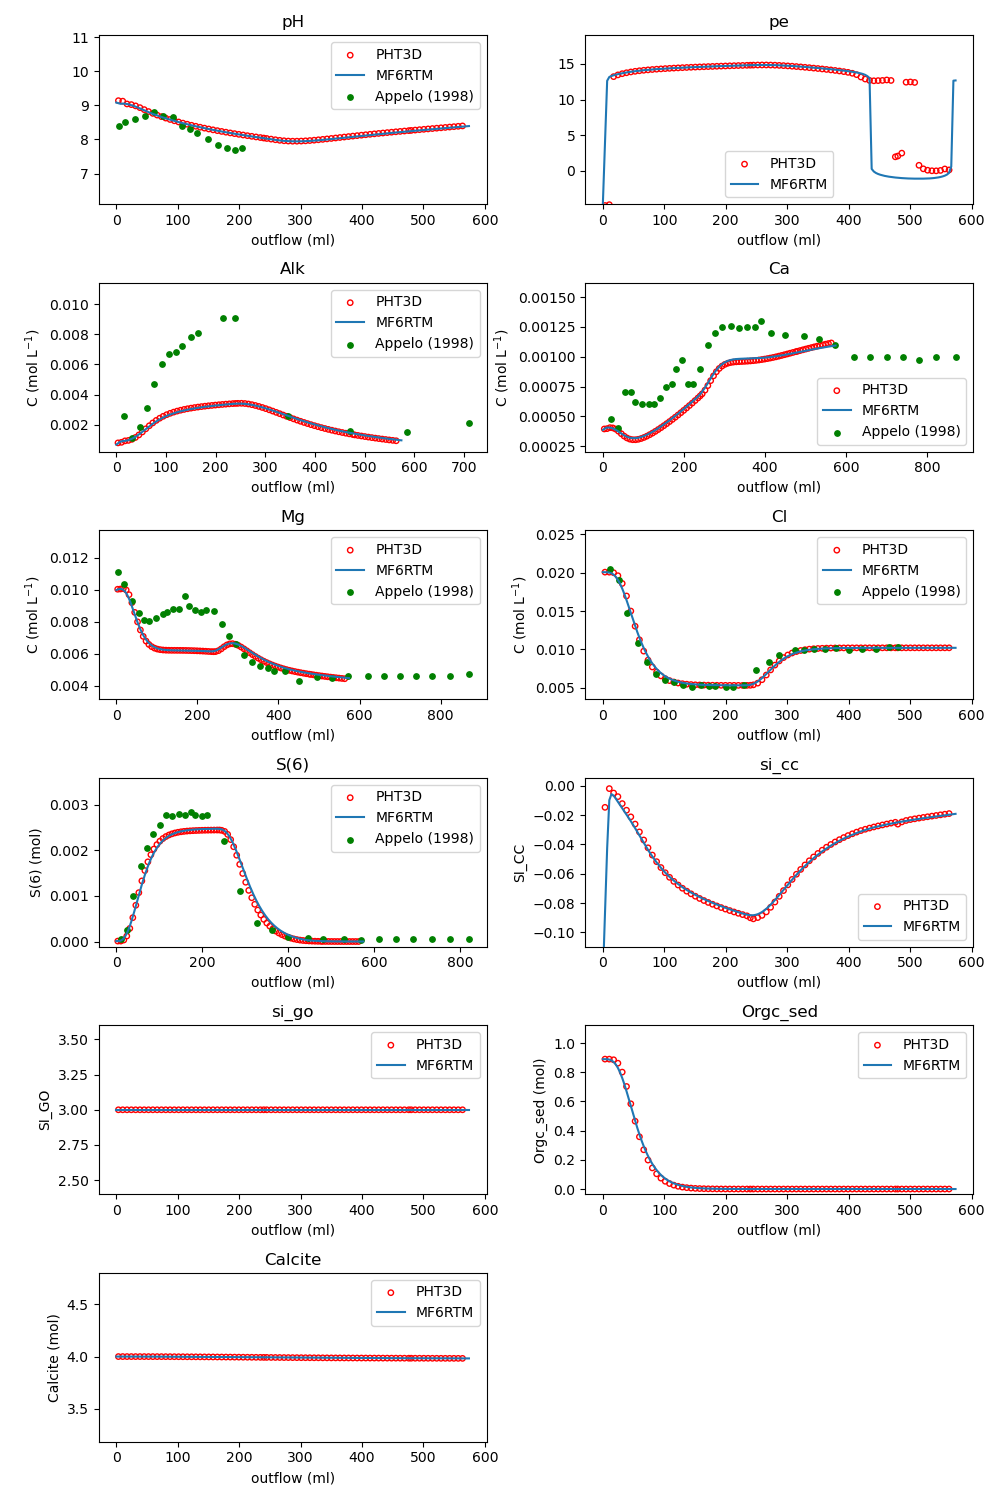
\includegraphics[width=\linewidth]{figures/ex5.png}
\caption{using a combination of equilibrium phases, kinetic and rates, cation exchange, and surface complexation. MF6RTM vs PHT3D and Tony Appelo 1998.}
\label{fig:ex5}
\end{figure}

\section{Main Issues}
MF6 transport, like MFUSG, has numerical dispersion that significantly influences reactions in some reactive transport cases. This is particularly important when reactions are sensitive to small changes in concentrations.
\section{Roadmap}

The following features are on the priority list for the roadmap:

\begin{enumerate}
    \item Finish coding autotests
    \item Two more complex 2D and 3D benchmarks.
    \item Test the LAK package for pit lake applications (money maker).
    \item Include DISV and the corresponding array bookkeeping.
    \item Add a scheme to call PHREEQC only when changes in concentration are above a threshold between time steps.
    \item Run a PESTPP-IES example using pyemu.
\end{enumerate}



\end{document}


